%%
%% This is file `mcmthesis-demo.tex',
%% generated with the docstrip utility.
%%
%% The original source files were:
%%
%% mcmthesis.dtx  (with options: `demo')
%%
%% -----------------------------------
%%
%% This is a generated file.
%%
%% Copyright (C)
%%     2010 -- 2015 by Zhaoli Wang
%%     2014 -- 2016 by Liam Huang
%%
%% This work may be distributed and/or modified under the
%% conditions of the LaTeX Project Public License, either version 1.3
%% of this license or (at your option) any later version.
%% The latest version of this license is in
%%   http://www.latex-project.org/lppl.txt
%% and version 1.3 or later is part of all distributions of LaTeX
%% version 2005/12/01 or later.
%%
%% This work has the LPPL maintenance status `maintained'.
%%
%% The Current Maintainer of this work is Liam Huang.
%%
\documentclass{mcmthesis}
\mcmsetup{CTeX = false,   % 使用 CTeX 套装时,设置为 true
        tcn = 2003684, problem = D,
        sheet = true, titleinsheet = true, keywordsinsheet = true,
        titlepage = true}
\usepackage{palatino}
\usepackage{mwe}
\usepackage{graphicx}
\usepackage{subcaption}
\usepackage{float}
\usepackage{multirow}
\usepackage{indentfirst}
\usepackage{gensymb}
\usepackage[ruled,lined,commentsnumbered]{algorithm2e}
\usepackage{geometry}
\usepackage{booktabs}
\usepackage{setspace}
\usepackage{listings}
\geometry{left=2cm,right=2cm,top=2cm,bottom=2cm} %%页边距

\begin{document}
\linespread{0.6} %%行间距
\setlength{\parskip}{0.5\baselineskip} %%段间距
\title{PnP: A Real-Time Passing Network - Player Combining Model}

\date{February 17, 2020}\begin{abstract}

    Soccer team the Huskies requires a mathematical model to evaluate the players' performance on teamwork and help the coach make structural strategies.

    To address the issue, the paper proposes the real-time passing network - player combining model ( PnP) that measures both players' individual and collective performances, which can help the coach decide the starting team formation before the match and make instant adjustments during the match.

    The PnP model consists of three sub-models: static passing network, player model and real-time passing network.

    The static passing network is a weighted directed graph where nodes are players and edges represent distance. The weight of edges involves the type and length of passes as well as players' positions. Pass clustering coefficient , a modification of clustering coefficient in graph theory, is introduced to measure a player's participation and indicate team performance. K-means clustering algorithm is applied to divide players into three levels. Finally the pass clustering coefficient is compared with the PageRank value to identify the better model.

    The player model is a comprehensive evaluating system, inspired by football games. It takes four major scores into account, namely shot, pass, defense and body. Each score contains several subscores computed by certain indices derived from raw data. Then, Analytic Hierarchy Process is employed to determine the weights of four major scores in different positions. These four scores form the total score. According to players' total scores in different positions, we define their types: offensive, defensive or organizational.

    Based on the player model and dyadic or triadic configuration given by the model, three different sets of team formation, respectively focusing on attack, defense, and organization, are recommended to the coach.

    The real-time passing network is a modification of the static passing network. Given a time parameter, it is able to screen out the statistics in certain time period and apply the same assessment as the static passing network to them.

    Based on the player model and dyadic or triadic configuration given by the model, three different sets of team formation, respectively focusing on attack, defense and organization are recommended to the coach. Besides, combined with player model, the real-time passing network is able to give the coach suggestions about substitutions. By analyzing the real-time passing network of the opponent and applying the min-cut algorithm, the model can provide the coach with more real-time defense strategies towards the opponent. The PnP model can also be generalized to improve teamwork in societies through proper analogy.

    The end of the paper represents the sensitivity analysis and discussion of strengths and weaknesses.
		\begin{keywords}
			clustering coefficient; PageRank; K-Means; AHP; min-cut
		\end{keywords}
	\end{abstract}

\maketitle

\tableofcontents

\newpage

\section{Introduction}	
\subsection{Problem Background}
In an interconnected society, it requires the coordination between people with diverse expertise to address complex issues. Competitive team sports like soccer are good illustrations of the situation. A team will function well only if players can effectively cooperate with teammates and fully take advantage of their features.

Coach is commonly considered as the person who decides how the ball should pass through players, but we should not neglect the role of data in the decision. Most European football clubs in premier leagues have data analysts in the coaching staff nowadays to evaluate players' performances and give advice to the coach. Mathematical model evaluation even becomes the determinant when Liverpool FC decides whether to sign a player \cite{Liverpool}. Therefore, it is necessary to devise a model to understand the team's dynamics and figure out the best configuration of the team.

\subsection{Our Work}

A successful coach should be good at both the tactical arrangement before the match and the on-the-spot adjustments, therefore, we consider the problem from two aspects:
\begin{itemize}
  \item To make proper arrangements, we need to evaluate the performance of the Huskies based on the historical data. The problem can be solved on two levels: teamwork and individual ability. In Section \ref{Passing Network}, we establish a passing network to evaluate the players' coordination mainly based on the passing data. Besides, teamwork
      should be the correct combinations of players with different features, so we devise a player model in Section \ref{Sec:single} to evaluate each player's ability using the events data.
  \item For on-the-spot adjustment, we modify the passing network, proposing real-time passing network in Section \ref{Sec:RTPN}, which can dynamically measure a player's performance during the match.
\end{itemize}

After the establishment of real-time passing network - player combining model, we show its effectiveness in Section \ref{Sec-Implementation}, further discuss the model in Section \ref{Sec-Analysis} and make conclusions in Section \ref{Sec-Conclusion}.

\section{Assumptions}\label{Sec-Assume}
\begin{enumerate}
	\item \textbf{Pass routes and acceleration routes are all straight lines.}

Admittedly, pass routes and acceleration route can be curves sometimes but generally speaking, straight pass and acceleration play a dominant role. Therefore, we can safely regard all of them as straight routes.
	
\item \textbf{Successful duels and pass mean those followed by teammate's action.}

It is reasonable that a player's duels and pass are considered successful if his teammates control the ball after his action.

\item \textbf{A player shoots in target when the goal keeper makes save attempts.}

There is no doubt that the goal keeper will make save attempts when a shot is within the goal range.

\item \textbf{Player scores hardly change in the next season.}

Since we have analyzed players' performance consistently throughout the last season, dramatic changes in player scores will not happen in the next season.
	
\end{enumerate}
\section{Notations}\label{Sec-Nomen}
The following table shows the notations we use in the model. We will clarify the definitions when the corresponding concepts first appear in the main body.
\begin{table}[htbp]
 \centering
 \begin{spacing}{1.19}

 \begin{tabular}{lcl}
  \toprule
  Symbol & Definition \\
  \midrule
 $G$ & Passing network \\
 $V$ & Set of nodes in the passing network\\
 $E$ & Set of edges in the passing network\\
 $\Delta t$ & Time period in real-time passing network\\
 $G_{r}(\Delta t)$ & Real-time passing network with parameter $\Delta t$\\
 $V_{r}(\Delta t)$ & Set of nodes in the real-time passing network with parameter $\Delta t$\\
 $E_{r}(\Delta t)$ & Set of edges in the real-time passing network with parameter $\Delta t$\\
 $n$ & Number of players in the passing network\\
 $\overline{x_i}$ & Average position of player $i$ on x axis\\
 $\overline{y_i}$  & Average position of player $i$ on y axis\\
 $N_{i,j}$ & Number of passes from player $i$ to $j$  \\
 $d_{i,j}^{t}$ & Pass times distance from player $i$ to $j$\\
 $d_{i,j}^{l}$ & Average pass length from player $i$ to $j$  \\
 $d_{i,j}^{c}$ & Average coordinate distance between player $i$ and $j$\\
 $w_{i,j}$ & Weight of the edge from player $i$ to $j$ in the network\\
 $c_{i}$ & Pass clustering coefficient of player $i$ in the network\\
 $\overline{c_{C}}$ & Average clustering coefficient of players in Group C\\
 $S^{t}_{i}$ & Total score of player $i$\\
 $S^{b}_{i}$ & Body score of player $i$\\
 $S^{d}_{i}$ & Defense score of player $i$\\
 $S^{p}_{i}$ & Pass score of player $i$\\
 $S^{s}_{i}$ & Shot score of player $i$\\


  \bottomrule
 \end{tabular}
 \end{spacing}
\end{table}

\section{Statement of our Model} \label{Sec-Model}
In this section, we will present all the details of PnP model. Using historical data of the 38 games, we establish a passing network model and player model to evaluate the players' collective and individual performance. Then we expand the passing network, deriving a real-time passing network, which can measure the players' current performances and help the coach make on-the-spot adjustments.

\begin{figure}[htbp]
  \centering
  \includegraphics[width=16cm]{figures/overview.png}
  \caption{The overview of PnP model}\label{overview}
\end{figure}

\subsection{The Passing Network}\label{Passing Network}
A key factor that reflects the coordination between players is the distribution of passes. We devise a basic passing network to show the team's overall passing performance in one match.

The passing network is a \textbf{weighted directed graph} $G=(V,E)$, where one node represents a player and an edge $(u\rightarrow v,w)$ is a pass route from player $u$ to player $v$. The weight of the edge $w$ will be calculated in the following subsection.
\subsubsection{Weight of Edges in the Passing Network}
The weight of the edges shows the distance between players, which is a combination of three different kinds of distances considering multiple features like the type of passes and players' positions.
\begin{itemize}
  \item \textbf{Pass times distance}

  \qquad Based on the given data, we can obtain $N_{i,j}$, the number of passes from player $i$ to $j$ in one match. If the number of passes between two players is larger, then their positions are more likely to be closer, since passes between defenders are much more than that from a defender to a forward. Therefore, we define the \textbf{pass times distance} from player $i$ to player $j$ as:

\begin{equation}\label{dt}
d_{i,j}^{t}=
\begin{cases}
  0, & \mbox{if } i=j \\
  \frac{1}{N_{i,j}}, & \mbox{if } i\ne j, N_{i,j} \ne 0 \\
  +\infty, & \mbox{if } i\ne j, N_{i,j} = 0
\end{cases}
\end{equation}
  \item \textbf{Average pass length}

 \qquad We can also get the length of passes from the data. To show the length of passes, we define the \textbf{average pass length vector} as:

$$
\overline{D_{i,j}^l} = \left[\overline{d_{i,j}^{head\ pass}}, \overline{d_{i,j}^{hand\ pass}},\overline{d_{i,j}^{high\ pass}},\overline{d_{i,j}^{simple\ pass}},\overline{d_{i,j}^{launch}},\overline{d_{i,j}^{cross}},\overline{d_{i,j}^{smart\ pass}}\right]
$$
where  $\overline{d_{i,j}^{Type}}$ is the average pass length of each type from player $i$ to $j$ in one match. The length of each pass is the Euclidean distance between the origin and the destination of the pass.

\qquad Simply combining the items of average pass length vector together cannot reflect the distance precisely, because the type of pass can reflect the distance between players to some extent. For example, a smart pass can give us more information about passing distance than a simple pass, and a high pass may provide more. As a result, we give the pass length coefficient vector:
 $$
\begin{aligned}
  K^l&=\left[\overline{k^{head\ pass}}, \overline{k^{hand\ pass}},\overline{k^{high\ pass}},\overline{k^{simple\ pass}},\overline{k^{launch}},\overline{k^{cross}},\overline{k^{smart\ pass}}\right]^T \\
    & = \frac{1}{6.7}[0.8, 0.6, 1.3, 1.0, 0.7, 1.2, 1.1]^T
\end{aligned}$$

\qquad The \textbf{average pass length} from player $i$ to player $j$ is:
\begin{equation}\label{ld}
  d_{i,j}^{l}=
  \begin{cases}
    \overline{D_{i,j}^l}K^l, & \mbox{if } N_{i,j}>0 \\
    +\infty & \mbox{if }N_{i,j}=0
  \end{cases}
\end{equation}

  \item \textbf{Average coordinate distance}

  \qquad The previous two kinds of distances only consider passes, which is not informative enough as the number of passes between two players may be limited. We take the average coordinates of player $i$ $(\overline{x_i},\overline{y_i})$  into account. The \textbf{average coordinate distance} between player $i$ and $j$ is the Euclidean distance between their average positions:
  \begin{equation}\label{cd}
    d_{i,j}^c = \sqrt{(\overline{x_i} - \overline{x_j})^2 + (\overline{y_i} - \overline{y_j})^2}
  \end{equation}
\end{itemize}

With Equation \eqref{dt}, Equation \eqref{ld}, and Equation \eqref{cd}, the \textbf{weight of the edge} from $i$ to $j$ is calculated by:
\begin{equation}\label{weight}
  w_{i,j} = \exp\left(\frac{1}{k_c \stackrel{\sim}{d_{i,j}^c} + k_l \stackrel{\sim}{d_{i,j}^l} + k_td_{i,j}^t}\right)
\end{equation}
where:
\begin{itemize}
  \item $k_t = 0.7, k_l = 0.1, k_c = 0.2$
  \item $\stackrel{\sim}{d_{i,j}^l} = \frac{d_{i,j}^l}{\max \limits_{i,j}\{d_{i,j}^l\}},\stackrel{\sim}{d_{i,j}^c} = \frac{d_{i,j}^c}{\max \limits_{i,j}\{d_{i,j}^c\}}$
\end{itemize}

Figure \ref{match1} shows the passing network of match 1. The size of nodes is related to the number of passes launched by the player while the thickness of edges is related to the weight.
\begin{figure}[htbp]
  \centering
  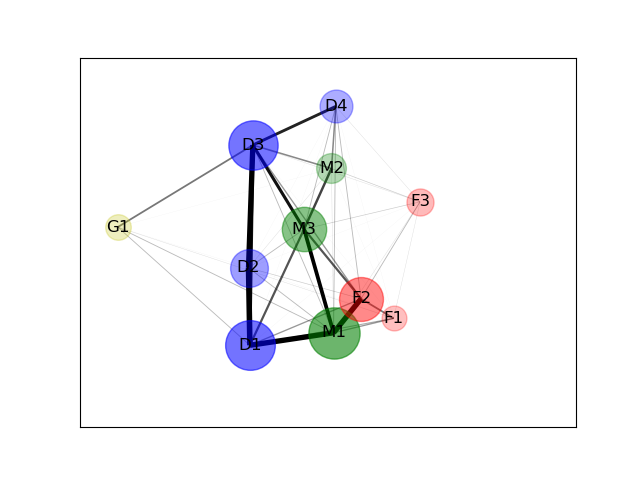
\includegraphics[width=10cm]{figures/match1.png}
  \caption{The passing network of match 1}\label{match1}
\end{figure}

\subsubsection{Pass Clustering Coefficient in the Passing Network}\label{Sec-ci}
Now we introduce \textbf{pass clustering coefficient}, which is a modification of the clustering coefficient in graph theory. Its original definition can be found in paper \cite{Coefficient}, measuring how well connected a node is to other nodes in the graph. Similarly, a high pass clustering coefficient in our network indicates a well-connected player in the team.

A non-weighted adjacency matrix $a_{i,j}$ is given here for convenience:$$
a_{i,j}=
\begin{cases}
  0, & \mbox{if } i=j \quad $or$ \quad  i\ne j,N_{i,j}=0\\
  1, & \mbox{if } i\ne j, N_{i,j} \textgreater 0
\end{cases}
$$
where $N_{i,j}$ is the number of passes from player $i$ to $j$.

Then the \textbf{degree} $k_{i}$ of a player(node) is $\sum_{i=1}^{n}a_{i,j}$.

Finally, we define the \textbf{pass clustering coefficient} of player $i$ as:
\begin{equation}\label{pcc}
  c_i =
  \begin{cases}
    \frac{1}{k_i(k_i-1)} \sum_{j,h} \frac{w_{j,i}+w_{i,h}}{2} a_{j,i}a_{i,h}a_{j,h}, & \mbox{if } k_i \geq 2 \\
    0, & \mbox{if } k_i \textless 2
  \end{cases}
\end{equation}

 To evaluate the effect of player $i$ in the team, we consider a situation in which player $j$ wants to pass the ball to  $h$ but cannot pass directly. Such situations often happen because of the opponents' defense or the far distance. As a result, player $i$ acts as an intermediary, forming a pass route $j \rightarrow i \rightarrow h$. The average weight of the route $\frac{w_{j,i}+w_{i,h}}{2}$ in Equation \eqref{pcc} reflects the engagement of player $i$ in the process. However, such route may not exist, so we introduce the adjacency indicator $a_{j,i}a_{i,h}$ to ensure its existence . Besides, if $a_{j,h}=0$, then it shows that player $j$ can not directly pass the ball to $h$, he has no choice but to pass the ball to another player. This kind of situation does not reflect active teamwork  and is eliminated by the introduction of $a_{j,h}$. The term $\frac{1}{k_i(k_i-1)}$ is based on the original definition of clustering coefficient in paper \cite{Coefficient}.

 \subsubsection{Pass Clustering Coefficient versus PageRank}
 The pass clustering coefficient $c_{i}$ can effectively measure one player's contribution to the team, making distinct difference between various levels of players. In fact, our initial thought about the passing network is a much simpler model, where the weight of the edges is just the number of passes and players are evaluated by the classic \textbf{PageRank} algorithm.

 PageRank is an algorithm to evaluate the influence of websites based on the hyperlinks between them. First proposed by Larry Page in 1999 \cite{PageRank}, PageRank algorithm becomes the core of the search engine giant, Google. The basic idea of PageRank is that if there are many hyperlinks point to a page, then the page should be influential and have a high PR(PageRank) value. Meanwhile, those pages that a page with high PR value points to should also also be influential and have high PR value. This idea generates from the impact factor of papers, as the most cited papers are most influential and have higher impact factors. The algorithm can also measure the influence of a node in the network, like a player's role in the team. We will apply both our passing network and the PageRank algorithm to the data of one match to show that the passing network suits the problem better.

 A mathematical method to find out the PR value is to calculate the eigenvector of the adjacency matrix $N_{i,j}$, but a more common-used method proposed in Larry's paper \cite{PageRank} is the \textbf{RandomWalk} model. A surfer will randomly jump from one page to another through hyperlinks. With the increase of visits, the frequency he visits a certain page will converge to a fixed value, which is defined as the PR value of the page. By iterating the frequency vector for a sufficient large of times, we can get the PR value of each page. We calculate the PR value of players based on the same idea. The PR value of player $x$ is given by:$$PR_{x}=(1-d)+d\sum \limits_{(y\rightarrow x,w)} \frac{w}{\sum_{(y \rightarrow z, w^{'})}w^{'}}PR_{y}$$
 where $d=0.95$ and we iterate the vector for 50 times. The code of the PageRank algorithm can be found in the Appendix ~\ref{a:pagerank}.

\begin{algorithm}
\caption{PageRank($epoch, d$)}
\ForEach{$x \in V$}{
    $pr_x \leftarrow 0$
    $sum_x \leftarrow 0$
}
\ForEach{$x, y \in V, (x \rightarrow y, w) \in E$} {
    $sum_x \leftarrow sum_x + w$
}
\While{$epoch > 0$}{
    $last \leftarrow pr$ \newline
    \ForEach{$x \in V$}{
        $res \leftarrow 0$ \newline
        \ForEach{$y \in V, (y \rightarrow x, w) \in E$} {
            $res \leftarrow res + w / sum_y * pr_y$
        }
        $pr_x \leftarrow (1 - d) + d * res$
    }
    $epoch \leftarrow epoch - 1$
}
\textbf{return} pr
\end{algorithm}

\begin{figure}[htp]
  \centering
  \includegraphics[width=16cm]{figures/pagerank.png}
  \caption{The pass clustering coefficient and PR value of players in match 10}\label{pagerank}
\end{figure}

Figure \ref{pagerank} shows the clustering coefficient $c_{i}$ and PR value of players in match10. We can see the distribution of $c_{i}$ covers a much larger range than the PR value, which will be very helpful for classifying players into three levels later. It can also be observed that defenders rank lower when they are measured by $c_{i}$, because we take into account the types of passes and the positions of players. Many passes of defenders are of minor importance as the ball is just hanging around in the backfield, not contributing to the team's coordination and goals. Compared with PageRank, the clustering coefficient is more in line with reality; it works better to evaluate a player's performance on teamwork.

\subsubsection{Classifying Players by K-Means Clustering Analysis} \label{K-means}
With the pass data of a whole game, we can calculate each player's pass clustering coefficient $c_{i}$. However, it is a local indicator that only measures one player. To obtain the overall information of the team, we study the average $c_{i}$ of all players and find that it is \textbf{positively related to} the result of the game. Meanwhile, we should consider the players' individual performance in the game to help coach make decisions.

To address these problems, we first divide the players into 3 groups A, B and C according to their $c_{i}$ in one match using \textbf{K-Means Cluster Analysis}. Note that these groups show relative relationships between players. For example, the average $c_{i}$ of Group A may vary greatly among different matches. Then we focus on the average $c_{i}$ of group C $\overline{c_{C}}$ and the number of players in Group A and Group C, which turn out to determine the result to a great extent.

K-Means clustering analysis is an unsupervised learning algorithm. The number of clusters $K$ is set manually. First, the algorithm randomly chooses $K$ samples from the dataset as the centers of the clusters. Then for each sample $x_{i}$, it will be distributed to the cluster whose center is closest to $x_{i}$. After this step, we will recalculate the center of each cluster. By repeating the two steps above until the centers of clusters do not change, the algorithm is finished.

\begin{algorithm}
\caption{K-Means($K, list, \varepsilon$)}
Randomly choose $K$ distinct items as initial $Center$: $Center_0, Center_1, ..., Center_{K-1}$ \newline
\While{\textbf{true}}{
    \ForEach{$x \in list$} {
        $dis \leftarrow +\infty$ \newline
        $pos = -1$ \newline
        \For{$i = 0$ to $K$} {
            \If{$Distance(x, Center_i) < dis$}{
                $dis \leftarrow Distance(x, Center_i)$ \newline
                $pos \leftarrow i$
            }
        }
        Insert $x$ in $BelongList_{pos}$
    }
    \For{$i = 0$ to $K$} {
        $NewCenter_i \leftarrow$ Average $(BelongList_i)$
    }
    \If{$\forall i$, $Distance (NewCenter_i, Center_i) < \varepsilon$} {
        \textbf{break}
    }
}
\textbf{return} $Center$
\end{algorithm}

We apply this algorithm to the players' pass clustering coefficients to evaluate their performances on teamwork in one match. Since different players' $c_{i}$ may vary by 10 times (as shown in Figure \ref{pagerank}), directly dividing the players into 3 clusters is not practical. Therefore, we first use K-Means to classify the players into 2 groups, Group A and others. Group A involves the players with the highest pass clustering coefficients, indicating that they are the key players in the network. We execute the same operation on the rest players, dividing them into Group B and C, where Group C consists of players with the lowest $c_{i}$. The average pass clustering coefficient of each group can give us information on the whole team's performance. We particularly focus on the \textbf{average pass clustering coefficient of Group C $\overline{c_{C}}$}, as we think that the players with the worst performance will  be the chance for opponents' attack. In fact, we find $\overline{c_{C}}$ is \textbf{positively related to} the result of the game, which will be further discussed in Section \ref{Sec-Implementation}.
\subsection{Player Model}\label{Sec:single}
Besides the players' performance on teamwork,  we also have to capture every player's individual abilities to arrange different formations according to the real situation. Therefore, we use the data provided to analyze both the player score and the player type.
\subsubsection{Player Score}
With the help of the data, we divide a player's ability into the following four aspects: \textbf{body}, \textbf{defense}, \textbf{pass}, \textbf{shot}. Figure \ref{player_score} demonstrates the specific components of the player score.
\begin{figure}[htbp]
  \centering
  \includegraphics[width=\textwidth]{figures/player_score.png}
  \caption{The components of the player score}\label{player_score}
\end{figure}
We have to mention that penalty is excluded from the shot score because we think it seldom happens and the kicker remains the same. Consequently, the penalty data has little influence on players' shot scores. What's more, we take no account of the goal keeper due to the difference of evaluating criteria between goal keepers and other players. For lack of the goal keeper's information, we can hardly figure out the real ability of the goal keeper. Moreover, goal keeper G1 is in the starting line-up of every match, indicating his priorities over other goal keepers.

For every sub-score of the player $i$, we find a decisive index $id$ and apply the same normalization formula to get a sub-score $\hat{s}^{id}_{i}$ between 0 to 1. Then, we just map $\hat{s}^{id}_{i}$ into $s^{id}_{i}$ , which ranges from 40 to 100, with Equation \eqref{wb}.
$$
    \hat{s}^{id}_{i}=\frac{id_{i}-\min \limits_{i}id_{i}}{\max \limits_{i}id_{i}-\min \limits_{i}id_{i}}
$$

\begin{equation}\label{wb}
    s^{id}_{i}=k\hat{s}^{id}_{i}+b
\end{equation}
where $k = 60, b = 40$.

Getting the sub-score, we determine the weight of each sub-score and integrate them into four main scores through the formula:
$$
    S^{ability}_{i} = \sum_{id}w_{id}s^{id}_{i}
$$

For simplicity, we list the index and weight of every sub-score in Figure \ref{sub-score}. After obtaining the four main scores, we use Equation \eqref{wd} to calculate the total score.
$$
    S^{t}_{i} = w_{b}S^{b}_{i}+w_{d}S^{d}_{i}+w_{p}S^{p}_{i}+w_{s}S^{s}_{i}
$$

\begin{figure}[htbp]
  \centering
  \includegraphics[width=\textwidth]{figures/subscore.png}
  \caption{The index and weight of each sub-score}\label{sub-score}
\end{figure}

To set the weight in Equation \eqref{wd}, we apply \textbf{Analytic Hierarchy Process(AHP)} \cite{AHP}. AHP is an especially effective way to decide on weight distribution when expert knowledge is provided. First, we construct the judgement matrix for defenders, midfielders and forwards.
\begin{center}
$J_{D} = \left[ {\begin{array}{*{20}{c}}
1 & 3 & \frac{3}{2} & \frac{2}{3} \\
\frac{1}{3} & 1 & \frac{1}{2} & \frac{1}{4} \\
\frac{3}{4} & 2 & 1 & \frac{1}{2} \\
\frac{3}{2} & 4 & 2 & 1
\end{array}} \right]$ $J_{M} = \left[ {\begin{array}{*{20}{c}}
1 & 2 & 2 & \frac{3}{2} \\
\frac{2}{3} & 1 & \frac{3}{2} & 1 \\
\frac{1}{2} & \frac{2}{3} & 1 & \frac{3}{4} \\
\frac{2}{3} & 1 & \frac{3}{2} & 1
\end{array}} \right]$ $J_{F} = \left[ {\begin{array}{*{20}{c}}
1 & \frac{1}{2} & 2 & 3 \\
2 & 1 & 3 & 4 \\
\frac{2}{3} & \frac{1}{3} & 3 & \frac{3}{2} \\
\frac{1}{2} & \frac{1}{4} & \frac{2}{3} & 1
\end{array}} \right]$
\end{center}
where the row(column) order is pass, shot, body and defense respectively.

Then, we normalize the three matrices and calculate the eigenvalues and feature vectors of them. Subsequently, we use the following two equations to calculate \textbf{Consistency index(CI)} and \textbf{CR}.
$$
    CI=\frac{\lambda_{max}-n}{n-1}
$$
$$
    CR=\frac{CI}{RI}
$$
where $n = 4, RI = 0.9$, and $\lambda_{max}$ means the maximum of all the eigenvalues.

Therefore, we get $CR_{D}=0.0118$ , $CR_{M}=0.0425$ , $CR_{F}=0.0738$ , which are all less than 0.1 , thus passing the consistency test. Finally, we get all the weights listed below in Table \ref{AHP_table}
\begin{table}[h]
    \centering
    \caption{AHP result}
    \label{AHP_table}
    \begin{tabular}{c c c c c}
\hline
    	Position & Pass Weight & Shot Weight & Body Weight & Defense Weight \\
\hline
	Defender & 0.288724 & 0.099053 & 0.204074 & 0.408148\\
	Midfielder & 0.368227 & 0.233279 & 0.165215 &0.233279\\
	Forward & 0.274037 & 0.45768 & 0.156978 & 0.111305\\
\hline
    \end{tabular}
\end{table}

We plug these weights into Equation \eqref{wd} . With Equation \eqref{wd}, we calculate and depict all the players' scores in different positions in Figure \ref{all_scores}.  If a player's any main score exceeds 80, it will be highlighted in green, which means this main score of the player has an obvious superiority over others'. Besides, the bold digit suggests that a player may be more competent in one position than others.
\begin{equation}\label{wd}
\left\{
             \begin{array}{lr}
             S^{t}_{i,D}=0.29S^{p}_{i} + 0.1S^{s}_{i} + 0.2S^{b}_{i} + 0.4S^{d}_{i}, &  \\
             S^{t}_{i,M}=0.37S^{p}_{i} + 0.23S^{s}_{i} + 0.17S^{b}_{i} + 0.23S^{d}_{i}, &  \\
             S^{t}_{i,F}=0.27S^{p}_{i} + 0.46S^{s}_{i} + 0.16S^{b}_{i} + 0.11S^{d}_{i}, &
             \end{array}
\right.
\end{equation}

\begin{figure}[htbp]
  \centering
  \includegraphics[width=\textwidth]{figures/all_scores.png}
  \caption{The index and weight of each sub-score}\label{all_scores}
\end{figure}

In short, Figure \ref{all_scores} gives us a comprehensive view on players' abilities and compares those scores in both personal and interpersonal perspective.

\subsubsection{Player Type}
After obtaining all the players' scores in different positions, we can further classify them into three types: \textbf{offensive, organizational} and \textbf{defensive} players. This is consistent with the bold digits in Figure \ref{all_scores}. To provide an intuitive view, we depict three player's scores in Figure \ref{three}. Those three players perform best compared with others in the same position. As we can see, they tend to have a relatively high score in any of the four domains. According to their features, we categorize D1 into defensive and organizational defender, M1 into organizational and defensive midfielder and F2 into offensive and organizational forward. For other players, we define their type in the same method. You can refer to Appendix \ref{score} for details.
\begin{figure}[htbp]\centering
\includegraphics[width=.3\textwidth]{D1_score.png}
\includegraphics[width=.3\textwidth]{M1_score.png}
\includegraphics[width=.3\textwidth]{F2_score.png}
\caption{Scores of three players}\label{three}
\end{figure}

With all the players' scores and types, we can offer the coach a deeper knowledge on the players and help him to form strategies either before or during a match, which will be discussed in Section \ref{Structual Strategy}.

\subsection{RTPN: Real-Time Passing Network}\label{Sec:RTPN}
\subsubsection{Definitions of RTPN and Real-Time Pass Clustering Coefficient}\label{Sec:RTPN1}
After building the static passing network of a match, we are able to  establish a dynamic one, which is named "\textbf{Real-Time Passing Network}" or \textbf{RTPN} in short. The RTPN is constructed by the data of last few moments. As a result, it indicates the current performance of every player. The network can also reflect the main passing group and formation of the team. With the help of the RTPN, we are able to analyze the data more dynamically.

To state formally, we define RTPN as a weighted directed graph $G_r(\Delta{t})$, where $\Delta{t}$ indicates the time period under consideration is $(t - \Delta{t}, t)$ supposing $t$ stands for the current time. Like other graphs, $G_r(\Delta{t})$ is constructed by its vertex set $V_r(\Delta{t})$ and edge set $E_r(\Delta{t})$. Its vertex set includes all the players who has participated in an event in the time period $(t-\Delta{t},t)$. Similarly, its edge set includes all the pass route in this time period. The weight on the edge is computed  with the same methods we stated above.

 With the RTPN built, we are able to calculate the \textbf{pass clustering coefficient} in the network. We use the same definition in Section \ref{Sec-ci} and use the same methods to compute it. The real-time clustering coefficient data in match 1 is shown in Figure \ref{tendency1}.

\begin{figure}[htbp]
    \centering
    \includegraphics[width=16cm]{figures/tendency_match1.png}
    \caption{The real-time clustering coefficient tendency in match 1}
    \label{tendency1}
\end{figure}

 We can infer a lot of information from this figure, which we will explain later in Section \ref{Sec:RTPNA}. In a word, like full-time clustering coefficient data, we can estimate the team performance and individual performance from it.

\subsubsection{Real-Time Strategies based on RTPN}\label{Sec:RTPN2}
After we estimate the performance data, we are able to give team coach suggestions about substitutions. Combined with the player model we have mentioned above, we can help the coach to choose the substitutes more precisely.

Our RTPN model be used to analyze both our players' performances and opponent's, We proposed following \textbf{RTPN-based strategies}:

\begin{itemize}
    \item \textbf{Attacking and Pass}: After estimating the performance data such as pass clustering coefficient in our RTPN, we are able to give team coach suggestions about substitutions. Combined with the player model we have mentioned above, we can help the coach to choose the substitutes more precisely.
    \item \textbf{Defense}: Use pass clustering coefficient in opponent's RTPN to analyze the core pass group of the opponent. If we could restrict their key player in the group, we might be able to reduce opponent's pass efficiency and control the game.
    \item \textbf{Defense}: The edge weights in our RTPN reflect the importance and frequency of the pass route. Sometimes it is not necessary and efficient to block all the heavy-weighted pass route. Since our goal is to prevent opponent from scoring, we believe if we can cut off the path from current ball-owner to the main forward, we are able to reduce opponent's goal to the utmost extent. The detailed methods will be explained in the next paragraph.
\end{itemize}

 Here we are going to discuss the last strategy we provide above. Our goal is to cut the path from current ball-owner to main forward of the opponent. We regard current ball-owner as the source of RTPN and main forward as sink of RTPN. The weights of edge in the RTPN can also be denoted as the flow of the edge. Thus, our strategy is to find the minimum-cut of the flow network. That is, find a node set $S$ satisfying:

$$
\begin{cases}
    S \subseteq V_r(\Delta{t}) \\
    source \in S \\
    sink \in V_r(\Delta{t}) - S
\end{cases}
$$

while minimizing:

$$
    \sum_{(u\rightarrow v, w) \in E_r(\Delta{t})}^{u \in S, v \in V_r(\Delta{t}) - S} w
$$

The problem can be solved easily with enumerate algorithm in a time complexity of $O(|E_r(\Delta{t})|\cdot 3^{|V_r(\Delta{t})|})$, since $|V_r(\Delta{t})|$ is small enough. If the size of $V_r(\Delta{t})$ become larger, we can use the Max-flow min-cut theorem \cite{Wiki_cut_theorem} to transform the problem into a maximum flow problem and use Dinic's Algorithm \cite{Wiki_Dinic} to solve it in a time complexity of $O(|V_r(\Delta{t})|^2\cdot |E_r(\Delta{t})|)$.


\section{Implementation} \label{Sec-Implementation}
With the accomplishment of the model construction, now we use the model to process the given data, demonstrating its effect. We will also propose corresponding strategies based on the analysis.
\subsection{Average Clustering Coefficient}\label{Sec-cc}
We calculate the \textbf{average clustering coefficient of Group C $\overline{c_{C}}$}  (introduced in Section \ref{K-means}) of all the 38 games through out the season, as shown in Figure \ref{cr7}.
\begin{figure}[htbp]
  \centering
  \includegraphics[width=16cm]{figures/coefficient_result.png}
  \caption{The relationship between $\overline{c_{C}}$ and the result}\label{cr7}
\end{figure}

We can observe a strong relationship between $\overline{c_{C}}$ and the result of the game. The team only lost one game among the games whose $\overline{c_{C}}$ is over 35 and only won one game among the 16 games whose $\overline{c_{C}}$ is under 15. It shows that more passes and less distinction between the players' performance are helpful to the team's victory.

However, for the games between this two levels, this indicator does not give a clear classification between victory and loss. The reason why this situation happens is that the passing network only processes the pass data. If a player is excellent at finishing but not so good at organizing, like Inzaghi, his contribution to the team may be underestimated in the passing network because of the relatively lower number of passes. This problem can be greatly alleviated by introducing our player model as it considers the comprehensive ability of a player, so \textbf{the combination of passing network and player model} will be the best solution.
\subsection{Pre-Match Structural Strategies}\label{Structual Strategy}
As is discussed in our model part, we can optimize our formation and player configuration either before or during a match with the analysis of individual model and passing network.

For lack of rival's concrete data, we cannot design a much too sophisticated strategy before a match; however, we can use our individual model to devise several sets of starting line-ups for different purposes. After researching every match's starting line-ups, we spot that there are altogether six sorts, which are 4-4-2, 4-3-3, 5-3-2, 4-5-1, 5-4-1 and 4-2-4, ranking in frequency from high to low. Combining individual abilities with players' preferred foot, we propose three distinct starting line-ups focusing on \textbf{organization (4-4-2)}, \textbf{attack (4-3-3)} and \textbf{defense (4-5-1)} respectively.
\begin{figure}[htbp]
  \centering
  \includegraphics[width=14cm]{figures/coordination.png}
  \caption{The players who make the best combination}\label{best}
\end{figure}

To determine the proper players, we should consider not only their individual ability but also their combination, so we study the players of Group A (the highest $c_{i}$)throughout the last season. The result shows that player M1 is the core of the team who launches most passes, while F2, M3 and M4 are also key players that dominate the passes. Moreover, there is a remarkable mutual pass relationship between either two or three of them. This \textbf{dyadic} or \textbf{triadic configuration} indicates their excellent teamwork.

As is depicted in Figure \ref{line-up}, we select eleven players for the organization formation based on all the factors mentioned above. We believe that those eleven players have stable performance and  make good teamwork. This formation aims to seek for \textbf{a balanced trade-off} between attack and defense; meanwhile, it also elevates the \textbf{pass accuracy} and \textbf{number of times}.

\begin{figure}[htbp]\centering
\includegraphics[width=.3\textwidth]{organization_formation.png}
\includegraphics[width=.3\textwidth]{attack_formation.png}
\includegraphics[width=.3\textwidth]{defense_formation.png}
\caption{Three line-ups}\label{line-up}
\end{figure}

For the attack formation, we replace M4 with F1 to improve the attacking capacity. Interestingly, we also substitute D4 for D5 though D5 possesses a higher score as a defender. We reckon that side defenders should also take an active part in attacking. Therefore, we choose D4, who belongs to \textbf{offensive defenders}, to reinforce our attacking ability.

For the defense formation, we add M8 to consolidate the defense of midfield. As you can see, we replace F2 and F4 with F6 because the acceleration score of F6 is the highest in forwards. When using the defense formation, we usually have to depend on quick counterattacks to goal; hence, a forward with \textbf{outstanding acceleration capacity} may play a crucial role in the defense formation.

We recommend that the coach apply attack formation as the starting line-up to weaker rivals, organization formation to equivalent ones and defense formation to stronger ones.

\subsection{The Application of Real-Time Passing Network}\label{Sec:RTPNA}
We have explained RTPN in Section \ref{Sec:RTPN1}. Here is an example of using RTPN to analyze match data. From Figure \ref{tendency1} we can infer the following conclusions:

\begin{itemize}
    \item In the beginning of the match, player M1 and D1 had high clustering coefficient, which indicates they had formed a core dyadic pass relation. Based on their positions, we infer that during this period, what our team mainly did was defense.
    \item During the center period of the first half, player F1, F2, D4 began to join the passing group, which made a triadic pass relation of player M1, D1, F2. We can verify our conclusion from Figure \ref{match1}. During this period, our team was mainly organizing and attacking.
    \item In the second half, the clustering coefficient of every player dropped owing to the lack of physical strength. Player M2, F1 and D4 began to have a high clustering coefficient, which indicates their attacking attempts were mainly in the wing side based on the average position in Figure \ref{match1}. What we also know is the substitution of the coach came into effects immediately.
\end{itemize}

From the conclusions above, we suggests that our RTPN is able to assist the team coach in decision-making by assessing the player performance and main pass group.

Analyzing our opponent's data can help us have a better understanding of our opponent's structures and strategies, which is vital for us to set counter-strategies.

\begin{figure}[htbp]
    \centering
    \includegraphics{figures/match5-o.png}
    \caption{The real-time passing network and pass clustering coefficient of opponent in match 5 (from 10 minutes to 20 minutes, the orange line stands for the min-cut plan)} \label{666}
\end{figure}

For example, we use our RTPN to analyze the opponent's data in match 5 from 10 minutes to 20 minutes. The data is shown in Figure \ref{666}. From the statistics we can know that the current pass group of opponent is D3, M1 and F2, and D3 is the core of this group. In order to limit opponent's performance, we can take the following measures:
\begin{itemize}
    \item Make some players cut off player D3's pass route, so that the group will disappear because player D3 is restricted.
    \item Keep the ball away from forward F2. Suppose the ball is controlled by D3 currently, then we can regard D3 as source and F2 as sink. Using our strategy in Section \ref{Sec:RTPN2}, we have to compute a min-cut from M1 to F2. After calculation, we find out the plan shown in Figure \ref{666} can minimize the cost. So we can make some players cut off these paths, so that F2 can not get the ball easily. As a result, the opponent's performance will be limited.
\end{itemize}

In short, our model can be applied during the match, it can provides the team coach with more information about opponent and give useful suggestions.

\subsection{Solutions to the tasks}
\begin{itemize}
  \item To identify the network patterns, we establish a passing network in Section \ref{Passing Network} evaluating the team in one match. We also propose the real-time passing network in Section \ref{Sec:RTPN} to measure players' instant performance.
  \item The pass clustering coefficient $c_{i}$ measures one player's coordination with teammates while the average clustering coefficient of Group C $\overline{c_{C}}$ can reflect the overall performance. More details can be found in Section \ref{Sec-ci} and Section \ref{Sec-cc}.
  \item By applying the player model and static passing network to the given data, we propose the strategies on team formation in Section \ref{Structual Strategy}. According to the analysis of the passing network, we suggest that the midfielder and right wing should be reinforced in the next season. Also, the coach should emphasize on teaming skills to make the partial cooperation more diverse. Besides, the real-time passing network can help the coach with substitutions and real-time strategies, which is discussed in Section \ref{Sec:RTPN2}.
  \item Based on our PnP model, we are able to propose a universal model of team performance and individual performance. The model is a combination of three sub-models, \textbf{the cooperation network model}, \textbf{the individual model} and \textbf{the real-time cooperation network model}.
    \begin{itemize}
        \item The first part, \textbf{the cooperation network}, which can indicate the total cooperation performance between every pair of team members, has a similar structure with our passing network. After redefining the weight of edges, we can also use PageRank and clustering coefficient to analyze individual performance, and use K-Means to divide team members into groups to analyze team performance and find out the core member of the group.
        \item  The second part, \textbf{the individual model}, which is based on all-time individual performance, is similar to our player model. We can use different indices, such as leadership, to analyze each member. After combining the indices together by certain methods like Analytic Hierarchy Process (AHP), we are able to find out the best position for every member in the team.
        \item The third part, \textbf{the real-time cooperation network model}, which is used to analyze the current team work performance of each member, is similar to our RTPN model. We reuse the definitions in the first model and use a time parameter $\Delta{t}$ to screen out those statistics out of time range; hence, we can analyze real-time performance and offer the team some suggestions on improving efficiency. If the team has an opponent, we can also use the network to analyze the opponent's performance and put forward some strategies to make our team more competitive.
    \end{itemize}
    This model can be used to analyze the team performance and individual performance most of the time. To generalize the model, we need to capture more aspects of teamwork such as the work procedure before a successful teamwork (the series of pass before successful shot or goal in soccer game). These aspects can provide us with a more direct way of judgement, which will improve our model and make it more general.
\end{itemize}


\section{Model Analysis}\label{Sec-Analysis}
\subsection{Sensitivity Analysis}
Our model contains several parameters. We determine some of the parameters through Analytic Hierarchy Process (AHP), some of them by knowledge in the literature, and other methods. In this section, we would like to produce a sensitivity analysis to show whether our model is sensitive to different values of parameters. We will choose the impact of an important parameters $\Delta{t}$ in our model as representative.

$\Delta{t}$ is a RTPN parameters with the meaning of the time period of the statistics. We set $\Delta{t}$ to 10 minutes in Section \ref{Sec:RTPNA}. Figure \ref{fig:sensative} shows the connection between different $\Delta{t}$ and real-time clustering coefficient of player M1 in match 1.

\begin{figure}[htbp]
    \centering
    \includegraphics[width=16cm]{figures/sensative1.png}
    \caption{The real-time clustering coefficient of player M1 in match 1 with different $\Delta{t}$}
    \label{fig:sensative}
\end{figure}

From the figure above we find that for all $\Delta{t}$, the curves reach their peaks in almost the same time. But when the time period $\Delta{t}$ is too short (e.g. $\Delta{t} = 5\ minutes$), some of the peaks disappear because the statistics are not enough for our RTPN to analyze player's performance. When the time period $\Delta{t}$ is too long (e.g. $\Delta{t} = 15\ minutes$), some peaks begin to combine with each other and the previous statistics and have a huge influence in current statistics and analysis, which makes our analysis not precise enough. In conclusion, our RTPN model is sensitive to its parameter $\Delta{t}$, and the setting of $\Delta{t}$ to 10 minutes is reasonable.

\subsection{Strengths and Weaknesses}
\subsubsection{Strengths}
\begin{enumerate}
\item Our model is based on scientific methods like \textbf{K-Means},\textbf{AHP} and \textbf{the min-cut model}, which make our model more reliable.
\item We modify the traditional clustering coefficient to fit our model and creatively integrate the individuality of players into their teamwork.
\item Various forms of figures are displayed to visualize our model.
\end{enumerate}
\subsubsection{Weaknesses}
\begin{enumerate}
\item When we calculate the weight of edges in the Passing Network, we take no account of the contribution it makes,such as leading to a goal.
\item For lack of opponents' data, our structural strategies before a match may not be flexible enough.
\end{enumerate}


\section{Conclusion} \label{Sec-Conclusion}
Our paper analyzes the previous match data of the Huskies to form a comprehensive awareness of both teamwork and personal features. Then we design the real-time passing network - player combining  (PnP) model consisting of three sub-models, namely Passing Network, Player Model and Real-Time Passing Network.

With the help of our model, we redefine the clustering coefficient and figure out its relation with team performance. Network patterns like partial cooperation between two or three players and structural strategies are also concerned.

We really hope our model and recommendation can be useful for both Huskies and teamwork in our society.
\newpage
    \bibliographystyle{IEEEtran}
    \bibliography{newrefs}

%\newpage
%\section*{Executive Summary}
	
%\noindent To whom it may concern,

\newpage

\begin{appendices}

\section{Edge Weight and Pass Clustering Coefficient Calculation} \label{a:edge}
\lstinputlisting[language=python]{pass_network_match.py}
\newpage
\section{PageRank Algorithm} \label{a:pagerank}
\lstinputlisting[language=python]{pagerank.py}
\newpage
\section{K-Means Clustering Algorithm} \label{a:kmeans}
\lstinputlisting[language=python]{kmeans_classification.py}
\newpage
\section{Scores of all players (The Overall and Detailed Version)} \label{score}
\begin{figure}[h]\centering
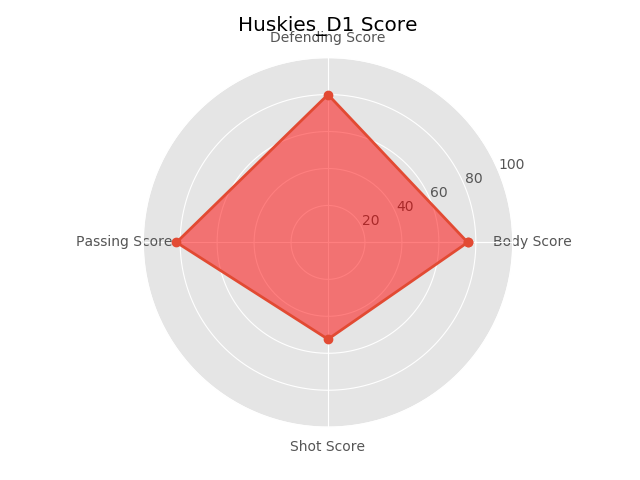
\includegraphics[width=.24\textwidth]{figures/pics-new/Huskies_D1_score.png}
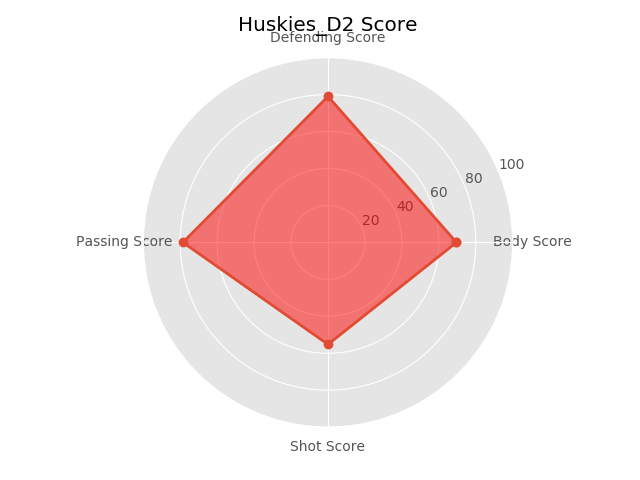
\includegraphics[width=.24\textwidth]{figures/pics-new/Huskies_D2_score.png}
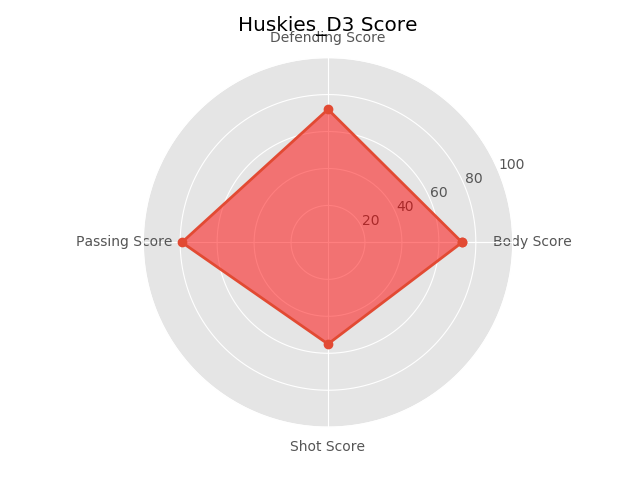
\includegraphics[width=.24\textwidth]{figures/pics-new/Huskies_D3_score.png}
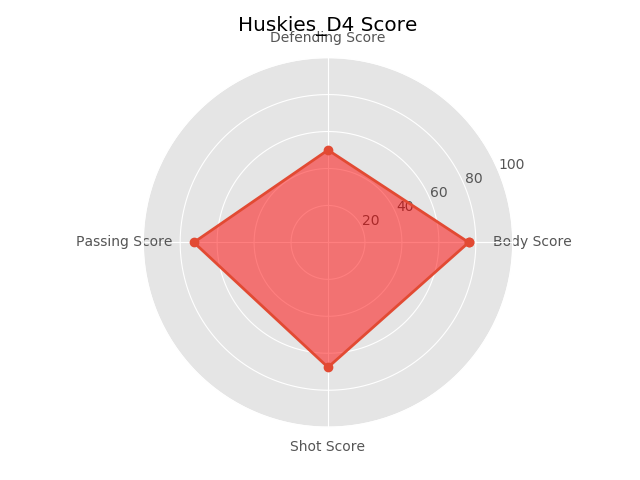
\includegraphics[width=.24\textwidth]{figures/pics-new/Huskies_D4_score.png}
\end{figure}
\begin{figure}[h]\centering
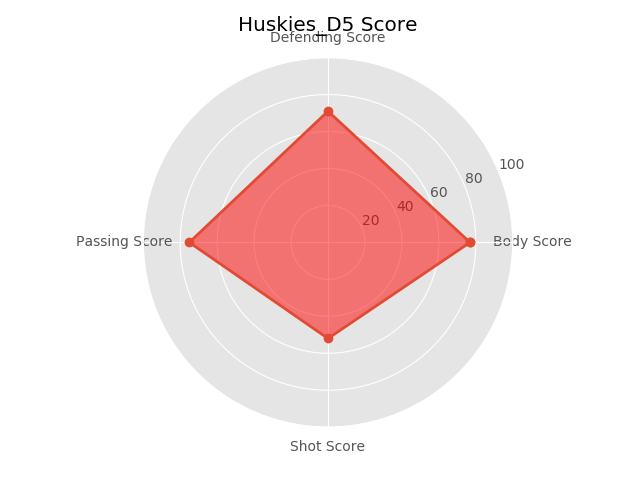
\includegraphics[width=.24\textwidth]{figures/pics-new/Huskies_D5_score.png}
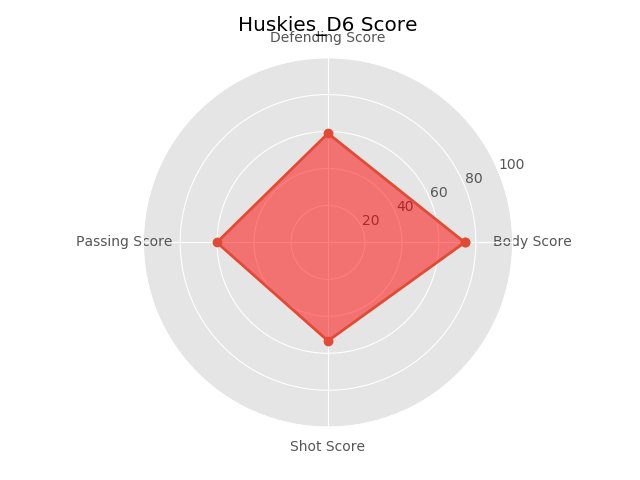
\includegraphics[width=.24\textwidth]{figures/pics-new/Huskies_D6_score.png}
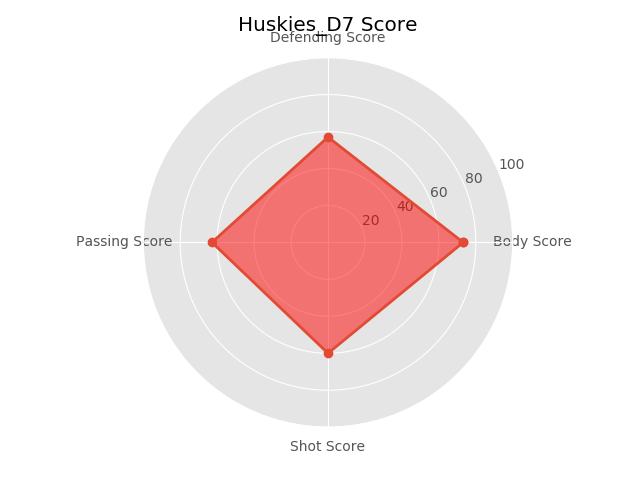
\includegraphics[width=.24\textwidth]{figures/pics-new/Huskies_D7_score.png}
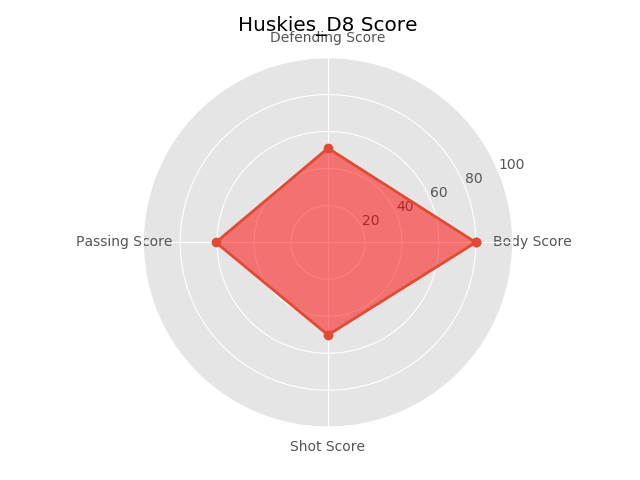
\includegraphics[width=.24\textwidth]{figures/pics-new/Huskies_D8_score.png}
\end{figure}
\begin{figure}[h]\centering
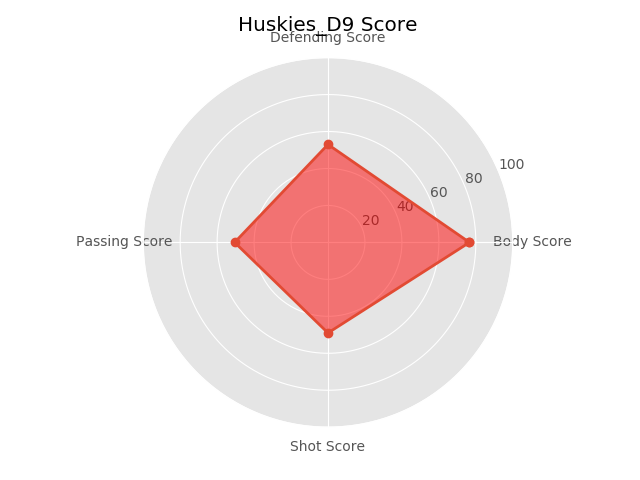
\includegraphics[width=.24\textwidth]{figures/pics-new/Huskies_D9_score.png}
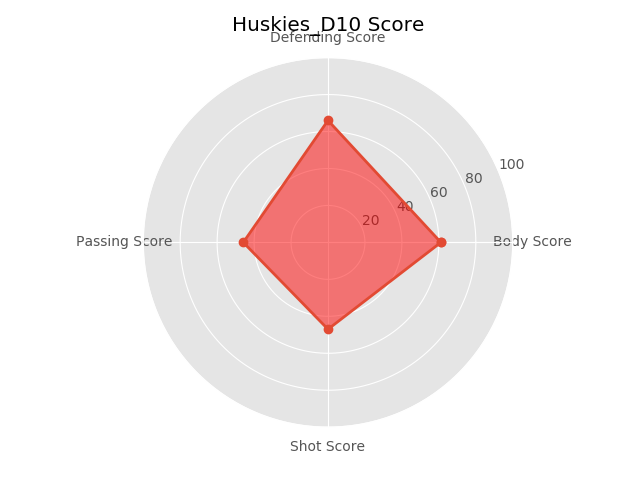
\includegraphics[width=.24\textwidth]{figures/pics-new/Huskies_D10_score.png}
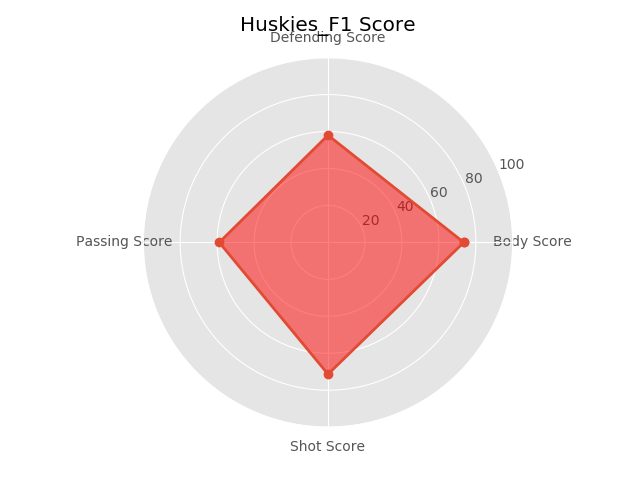
\includegraphics[width=.24\textwidth]{figures/pics-new/Huskies_F1_score.png}
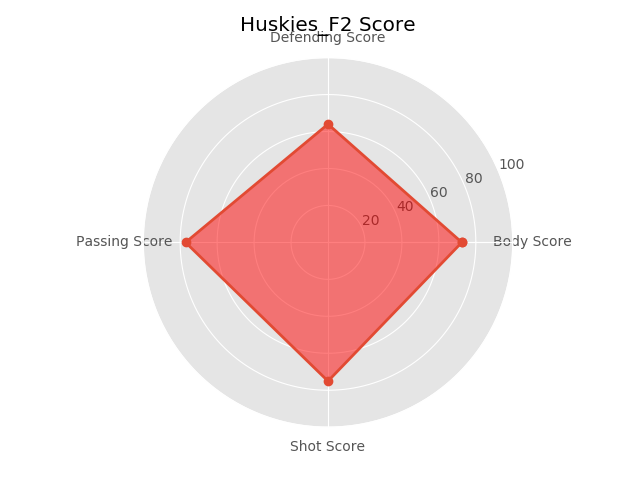
\includegraphics[width=.24\textwidth]{figures/pics-new/Huskies_F2_score.png}
\end{figure}
\begin{figure}[h]\centering
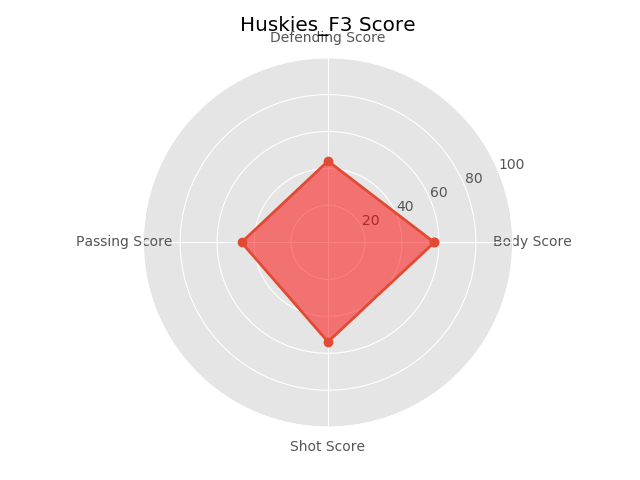
\includegraphics[width=.24\textwidth]{figures/pics-new/Huskies_F3_score.png}
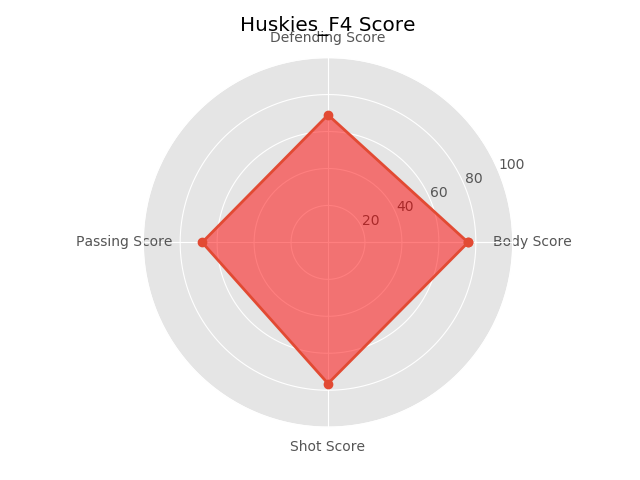
\includegraphics[width=.24\textwidth]{figures/pics-new/Huskies_F4_score.png}
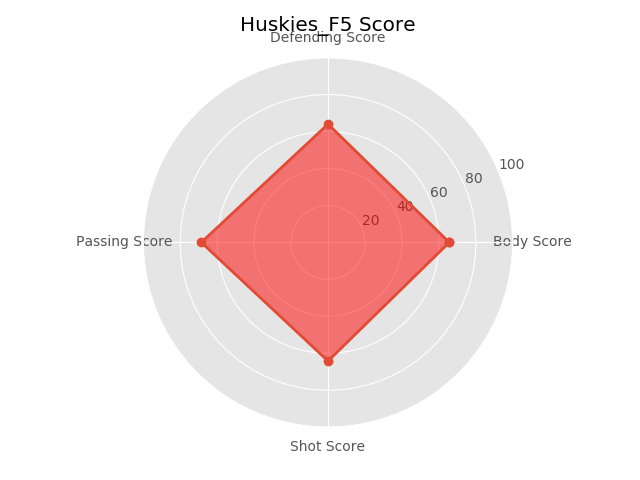
\includegraphics[width=.24\textwidth]{figures/pics-new/Huskies_F5_score.png}
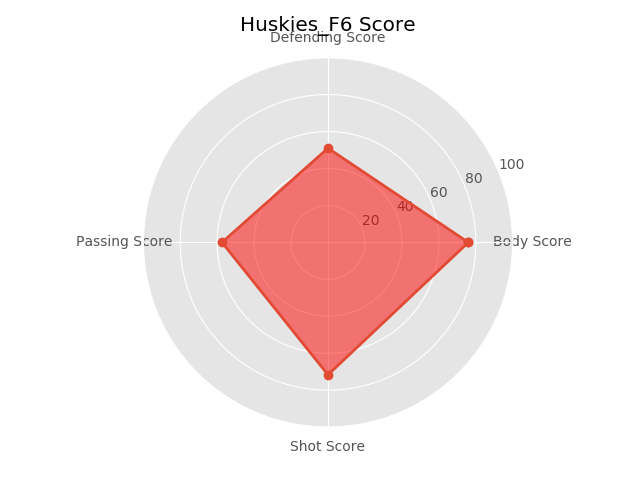
\includegraphics[width=.24\textwidth]{figures/pics-new/Huskies_F6_score.png}
\end{figure}
\begin{figure}[h]\centering
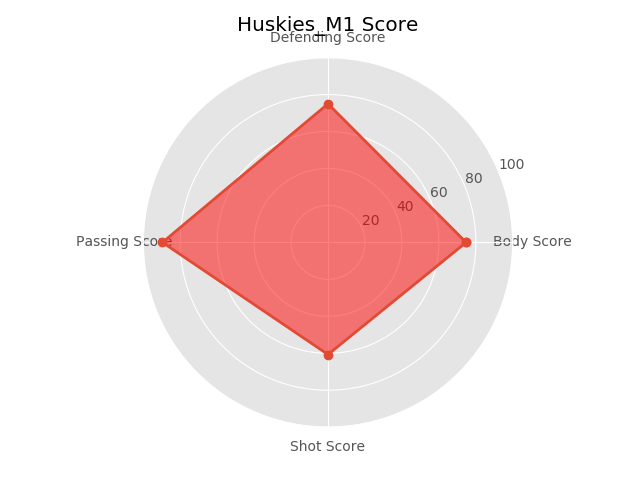
\includegraphics[width=.24\textwidth]{figures/pics-new/Huskies_M1_score.png}
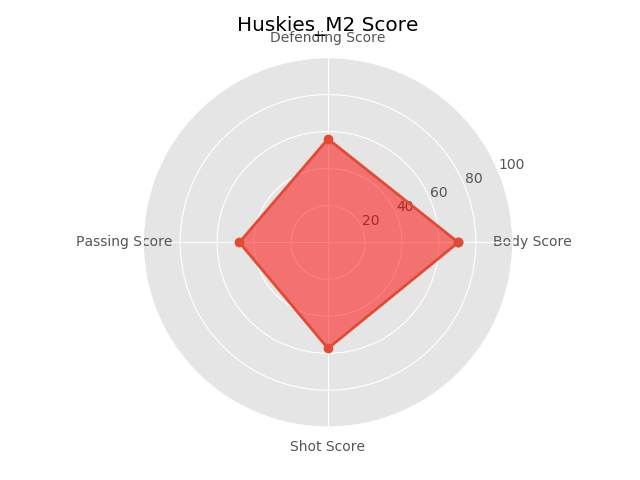
\includegraphics[width=.24\textwidth]{figures/pics-new/Huskies_M2_score.png}
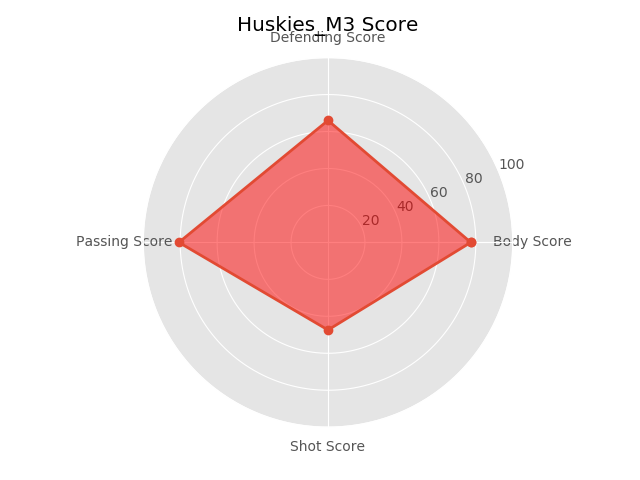
\includegraphics[width=.24\textwidth]{figures/pics-new/Huskies_M3_score.png}
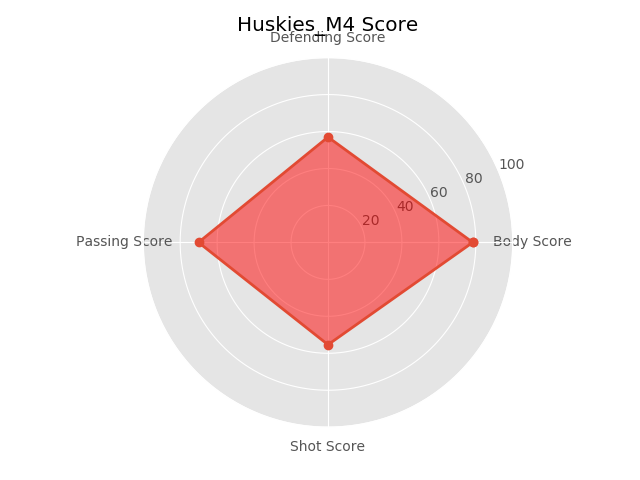
\includegraphics[width=.24\textwidth]{figures/pics-new/Huskies_M4_score.png}
\end{figure}
\begin{figure}[h]\centering
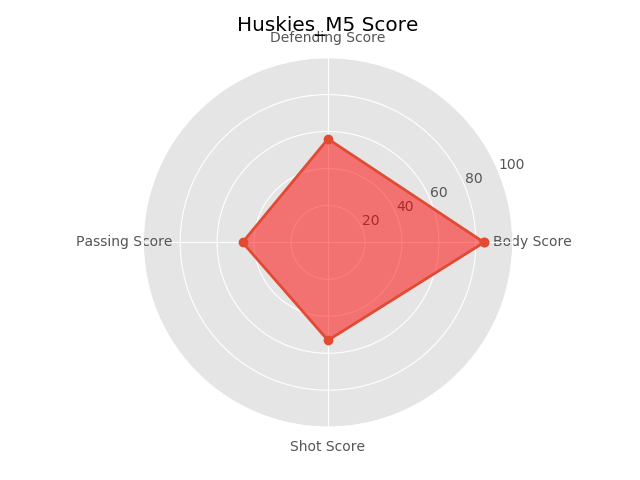
\includegraphics[width=.24\textwidth]{figures/pics-new/Huskies_M5_score.png}
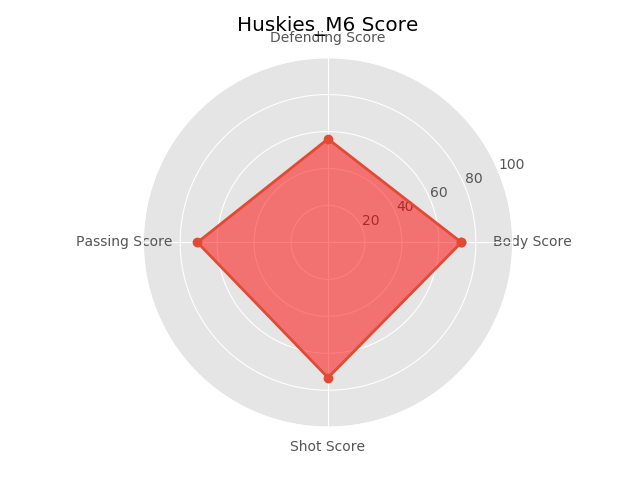
\includegraphics[width=.24\textwidth]{figures/pics-new/Huskies_M6_score.png}
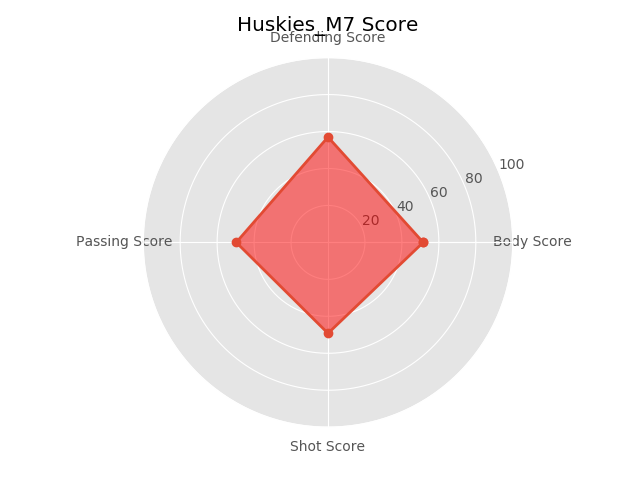
\includegraphics[width=.24\textwidth]{figures/pics-new/Huskies_M7_score.png}
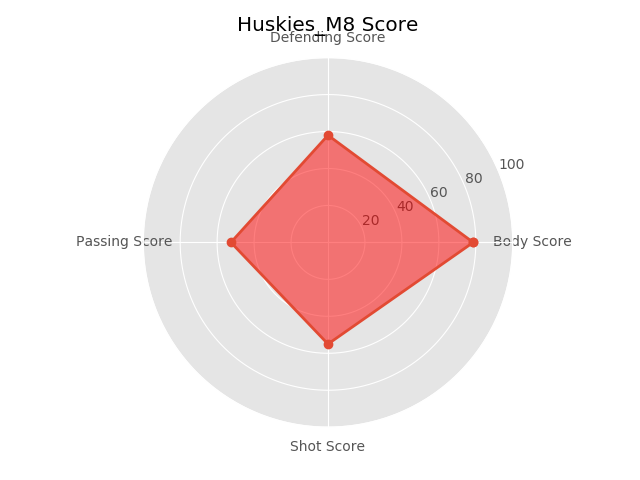
\includegraphics[width=.24\textwidth]{figures/pics-new/Huskies_M8_score.png}
\end{figure}
\begin{figure}[h]\centering
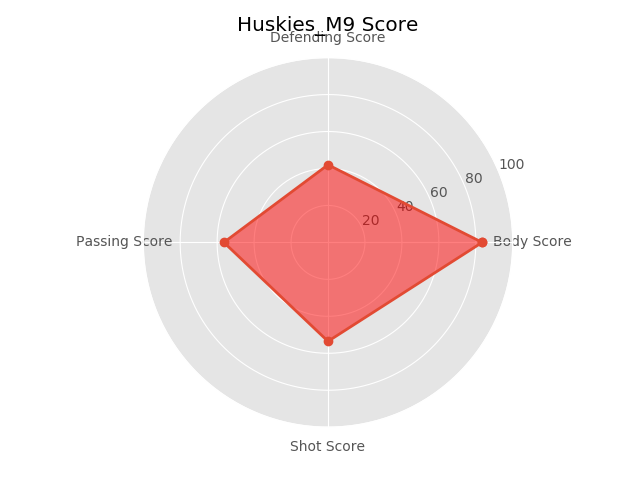
\includegraphics[width=.24\textwidth]{figures/pics-new/Huskies_M9_score.png}
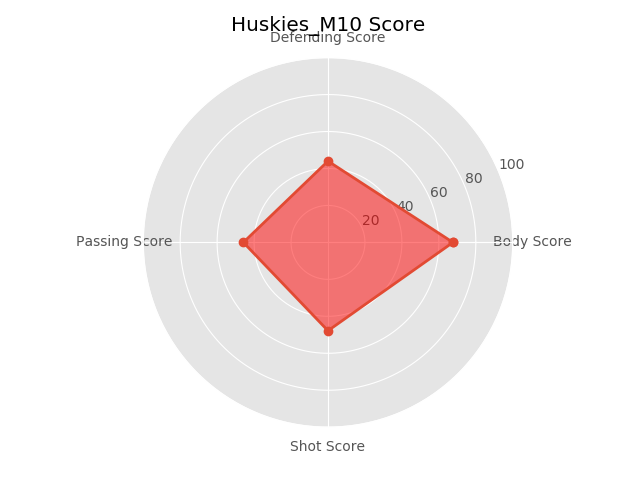
\includegraphics[width=.24\textwidth]{figures/pics-new/Huskies_M10_score.png}
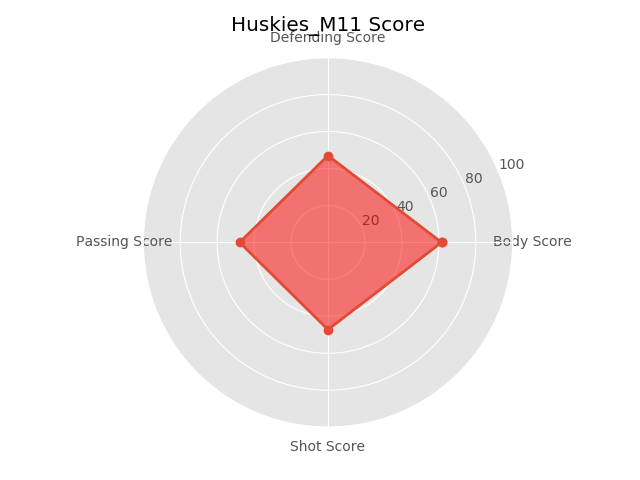
\includegraphics[width=.24\textwidth]{figures/pics-new/Huskies_M11_score.png}
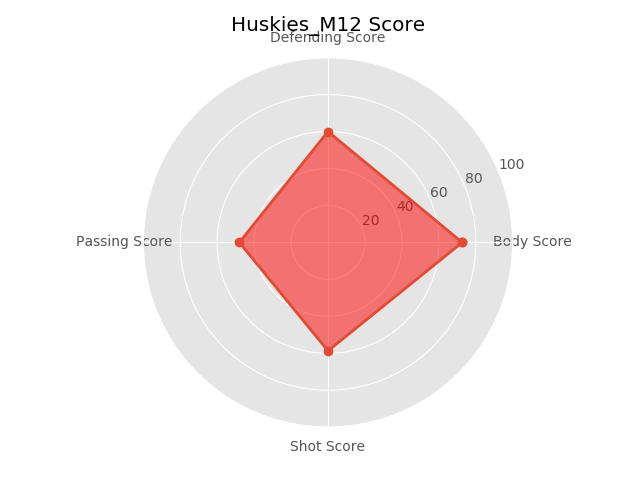
\includegraphics[width=.24\textwidth]{figures/pics-new/Huskies_M12_score.png}
\end{figure}
\begin{figure}[h]
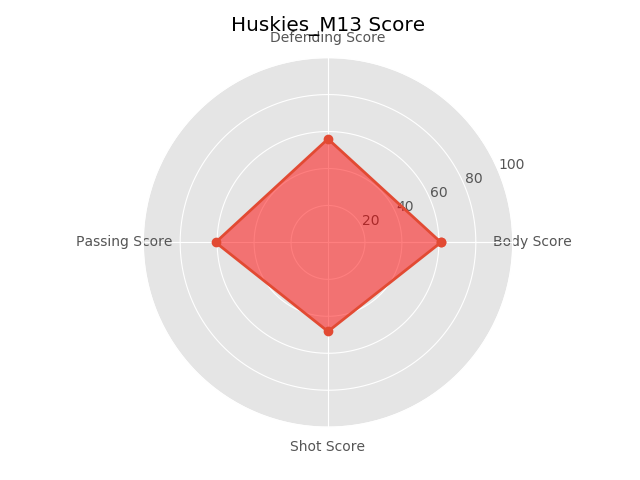
\includegraphics[width=.24\textwidth]{figures/pics-new/Huskies_M13_score.png}
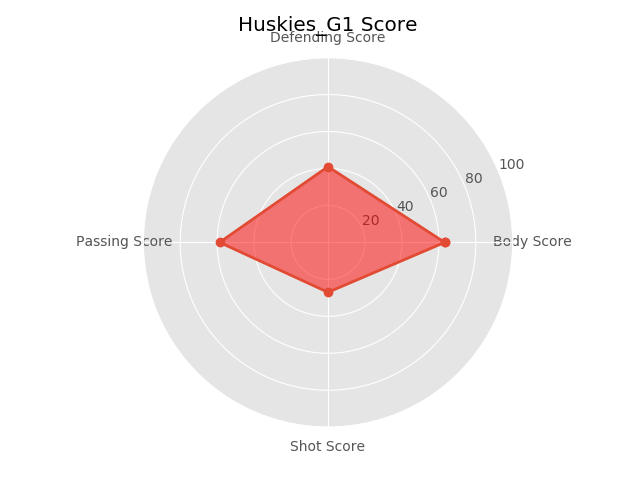
\includegraphics[width=.24\textwidth]{figures/pics-new/Huskies_G1_score.png}
\end{figure}

\begin{figure}[h]\centering
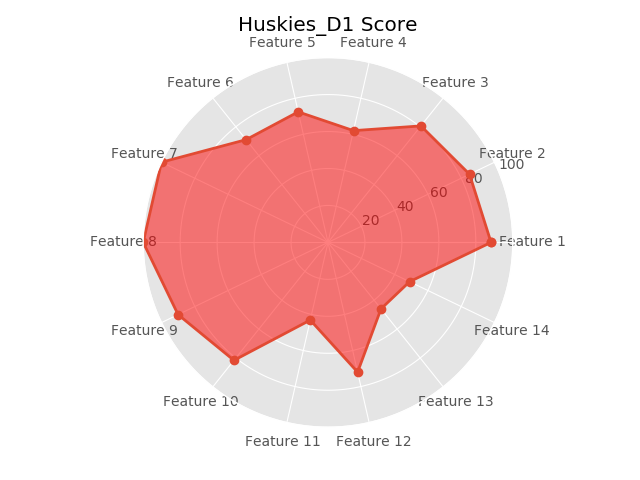
\includegraphics[width=.24\textwidth]{figures/pics-new/Huskies_D1_score_detail.png}
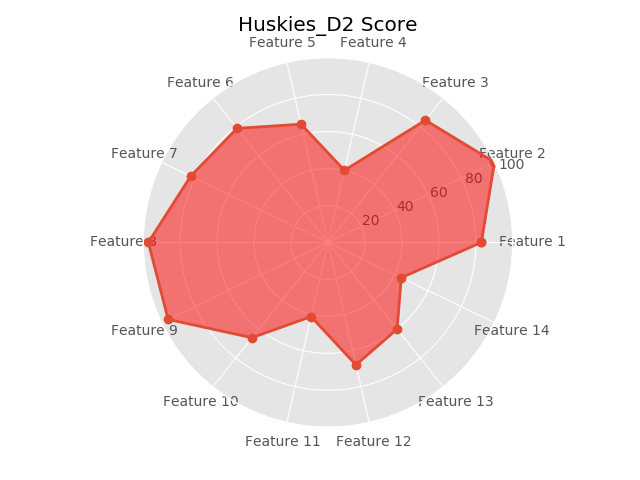
\includegraphics[width=.24\textwidth]{figures/pics-new/Huskies_D2_score_detail.png}
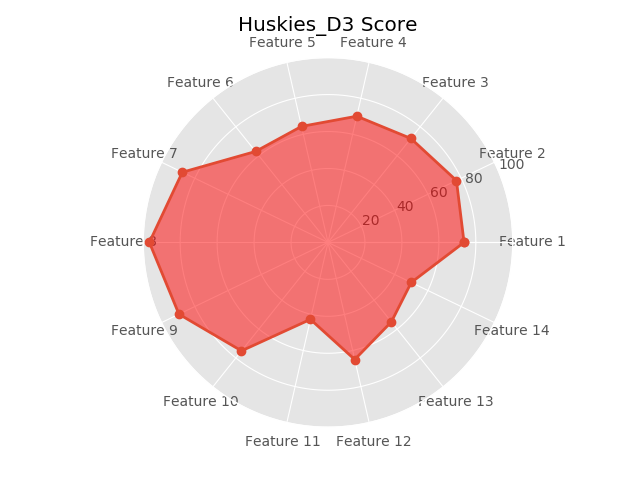
\includegraphics[width=.24\textwidth]{figures/pics-new/Huskies_D3_score_detail.png}
\includegraphics[width=.24\textwidth]{figures/pics-new/Huskies_D4_score_detail.png}
\end{figure}
\begin{figure}[h]\centering
\includegraphics[width=.24\textwidth]{figures/pics-new/Huskies_D5_score_detail.png}
\includegraphics[width=.24\textwidth]{figures/pics-new/Huskies_D6_score_detail.png}
\includegraphics[width=.24\textwidth]{figures/pics-new/Huskies_D7_score_detail.png}
\includegraphics[width=.24\textwidth]{figures/pics-new/Huskies_D8_score_detail.png}
\end{figure}
\begin{figure}[h]\centering
\includegraphics[width=.24\textwidth]{figures/pics-new/Huskies_D9_score_detail.png}
\includegraphics[width=.24\textwidth]{figures/pics-new/Huskies_D10_score_detail.png}
\includegraphics[width=.24\textwidth]{figures/pics-new/Huskies_F1_score_detail.png}
\includegraphics[width=.24\textwidth]{figures/pics-new/Huskies_F2_score_detail.png}
\end{figure}
\begin{figure}[h]\centering
\includegraphics[width=.24\textwidth]{figures/pics-new/Huskies_F3_score_detail.png}
\includegraphics[width=.24\textwidth]{figures/pics-new/Huskies_F4_score_detail.png}
\includegraphics[width=.24\textwidth]{figures/pics-new/Huskies_F5_score_detail.png}
\includegraphics[width=.24\textwidth]{figures/pics-new/Huskies_F6_score_detail.png}
\end{figure}
\begin{figure}[h]\centering
\includegraphics[width=.24\textwidth]{figures/pics-new/Huskies_M1_score_detail.png}
\includegraphics[width=.24\textwidth]{figures/pics-new/Huskies_M2_score_detail.png}
\includegraphics[width=.24\textwidth]{figures/pics-new/Huskies_M3_score_detail.png}
\includegraphics[width=.24\textwidth]{figures/pics-new/Huskies_M4_score_detail.png}
\end{figure}
\begin{figure}[h]\centering
\includegraphics[width=.24\textwidth]{figures/pics-new/Huskies_M5_score_detail.png}
\includegraphics[width=.24\textwidth]{figures/pics-new/Huskies_M6_score_detail.png}
\includegraphics[width=.24\textwidth]{figures/pics-new/Huskies_M7_score_detail.png}
\includegraphics[width=.24\textwidth]{figures/pics-new/Huskies_M8_score_detail.png}
\end{figure}
\begin{figure}[h]\centering
\includegraphics[width=.24\textwidth]{figures/pics-new/Huskies_M9_score_detail.png}
\includegraphics[width=.24\textwidth]{figures/pics-new/Huskies_M10_score_detail.png}
\includegraphics[width=.24\textwidth]{figures/pics-new/Huskies_M11_score_detail.png}
\includegraphics[width=.24\textwidth]{figures/pics-new/Huskies_M12_score_detail.png}
\end{figure}
\begin{figure}[h]
\includegraphics[width=.24\textwidth]{figures/pics-new/Huskies_M13_score_detail.png}
\includegraphics[width=.24\textwidth]{figures/pics-new/Huskies_G1_score_detail.png}
\end{figure}
\end{appendices}
\end{document}

%%
%% This work consists of these files mcmthesis.dtx,
%%                                   figures/ and
%%                                   code/,
%% and the derived files             mcmthesis.cls,
%%                                   mcmthesis-demo.tex,
%%                                   README,
%%                                   LICENSE,
%%                                   mcmthesis.pdf and
%%                                   mcmthesis-demo.pdf.
%%
%% End of file `mcmthesis-demo.tex'.
